%\documentclass[12pt,spanish,fleqn,openany,letterpaper,pagesize]{scrbook}

\usepackage[utf8]{inputenc}
\usepackage[spanish]{babel}
\usepackage{fancyhdr}
\usepackage{epsfig}
\usepackage{epic}
\usepackage{eepic}
\usepackage{amsmath}
\usepackage{threeparttable}
\usepackage{amscd}
\usepackage{here}
\usepackage{graphicx}
\usepackage{lscape}
\usepackage{tabularx}
\usepackage{subfigure}
\usepackage{longtable}


\usepackage{rotating} %Para rotar texto, objetos y tablas seite. No se ve en DVI solo en PS. Seite 328 Hundebuch
                        %se usa junto con \rotate, \sidewidestable ....


\renewcommand{\theequation}{\thechapter-\arabic{equation}}
\renewcommand{\thefigure}{\textbf{\thechapter-\arabic{figure}}}
\renewcommand{\thetable}{\textbf{\thechapter-\arabic{table}}}


\pagestyle{fancyplain}%\addtolength{\headwidth}{\marginparwidth}
\textheight22.5cm \topmargin0cm \textwidth16.5cm
\oddsidemargin0.5cm \evensidemargin-0.5cm%
\renewcommand{\chaptermark}[1]{\markboth{\thechapter\; #1}{}}
\renewcommand{\sectionmark}[1]{\markright{\thesection\; #1}}
\lhead[\fancyplain{}{\thepage}]{\fancyplain{}{\rightmark}}
\rhead[\fancyplain{}{\leftmark}]{\fancyplain{}{\thepage}}
\fancyfoot{}
\thispagestyle{fancy}%


\addtolength{\headwidth}{0cm}
\unitlength1mm %Define la unidad LE para Figuras
\mathindent0cm %Define la distancia de las formulas al texto,  fleqn las descentra
\marginparwidth0cm
\parindent0cm %Define la distancia de la primera linea de un parrafo a la margen

%Para tablas,  redefine el backschlash en tablas donde se define la posici\'{o}n del texto en las
%casillas (con \centering \raggedright o \raggedleft)
\newcommand{\PreserveBackslash}[1]{\let\temp=\\#1\let\\=\temp}
\let\PBS=\PreserveBackslash

%Espacio entre lineas
\renewcommand{\baselinestretch}{1.1}

%Neuer Befehl f\"{u}r die Tabelle Eigenschaften der Aktivkohlen
\newcommand{\arr}[1]{\raisebox{1.5ex}[0cm][0cm]{#1}}

%Neue Kommandos
\usepackage{Befehle}


%Trennungsliste
\hyphenation {Reaktor-ab-me-ssun-gen Gas-zu-sa-mmen-set-zung
Raum-gesch-win-dig-keit Durch-fluss Stick-stoff-gemisch
Ad-sorp-tions-tem-pe-ra-tur Klein-schmidt
Kohlen-stoff-Mole-kular-siebe Py-rolysat-aus-beu-te
Trans-port-vor-gan-ge}

%
%\begin{document}
%
\justifying

\chapter{Generalización espacial de modelos epidemiológicos basada en el
        concepto de Distancia Ambiental Normalizada NED}

  \par Los modelos temporales descriptos en capítulos anteriores se basan en la
    generación de relaciones empíricas entre datos ambientales derivados de
    información satelital y los datos de campo, correspondientes a los del vector
    propiamente dicho. Esto significa que sólo pueden construirse modelos en
    lugares donde esté disponible la información de campo, problema que se
    menciona al concluir el capítulo anterior.

  \par En ese marco, y con el objetivo final de mejorar la aplicación operativa
    presentada por Porcasi y colaboradores en 2012 \cite{porcasi_operative},
    en este capítulo se plantea el objetivo específico de generar
    una metodología para espacializar los datos contruidos siguiendo la
    metodología del capítulo anterior, basada en el concepto de
    \textbf{\textit{Distancia Ambiental Normalizada}} (NED).

\section{Descripción del problema}
  \par A partir de la disponibilidad de datos de campo en $N$ localidades
    diferentes, se generan
    $N$ modelos que relacionan la oviposición con variables ambientales
    derivadas de datos satelitales (\textit{lst\_night}, \textit{lst\_day},
    \textit{ndvi}, \textit{ndwi}, \textit{prec}). Por simplicidad, sin pérdida
    de generalidad, supongamos que dichos modelos son lineales:
    \begin{align}
      ovip_{j} = \beta_{j} + \sum{}{coef_{ji} \times envVar_{i}(j)}
    \end{align}

  \par Donde $coef_{ji}$ representa los coeficientes del modelo de la
    ciudad $j$ para la variable $i$, y $envVar_{i}(j)$ representa la variable
    ambiental $i$ evaluada en la posición correspondiente a la ciudad $j$.
    Es decir que para cada ciudad $j$, hay un conjunto diferente de
    coeficientes, que son aquellos que generan un ajuste óptimo de los datos
    disponibles. Aquí se denominan a estos $N$ modelos: $M_{1},\ M_{2},\ \dots,\ M_{N}$.


  \par Así, el problema que se plantea es aquel en el que el modelo se
    debiera utilizar en una nueva ciudad (no incluida en las $N$ anteriores) en
    donde se quiere obtener una estimación de la abundancia del vector; para
    de esa manera, obtener la estimación mencionada para cualquier otra
    ciudad. En particular en este caso, en la región norte de Argentina donde
    no se disponga de datos de campo.


  \par La idea más simple para extrapolar los modelos obtenidos sería usar,
    para un punto/pueblo adicional localizado en la posición $X$, un modelo $M_{X}$
    igual al modelo conocido de la ciudad más cercana geográficamente (vecino más cercano) es
    decir $M_{X}\ =\ M_{J}$ donde $J$ corresponde a la ciudad más cercana.
    Una mejora a este enfoque, es utilizar un promedio de los $N$ modelos conocidos
    ponderados por el inverso de la distancia de este nuevo punto $X$ a cada una
    de las ciudades $J$ donde se dispone de un modelo. Es decir, el modelo de la
    ciudad más cercana pesará más y el de la más alejada pesará menos, es decir:

    \begin{align}
      M_{X} = \sum{}{\frac{M_{j}}{L_{j}}} \label{Eq:dist}
    \end{align}

    donde $L_{j}$ representa la distancia normalizada de la ciudad $J$ a
    $X$ (en términos de la localización geográfica de la nueva ciudad).


  \par El problema de las soluciones anteriores, es que en realidad es más
    razonable pensar que el comportamiento de la población del vector/mosquito
    en una ciudad en el punto $X$ será más coincidente con una que se encuentre
    en una ciudad que sea más similar \textbf{ambientalmente} y no necesariemente
    con aquella que está más cerca geográficamente. En ese sentido, se debería
    utilizar (en el esquema de vecino más cercano) el modelo de la ciudad $J$
    que posea el medio ambiente más similar al del punto $X$. En otras palabras,
    así como ``más cerca", significa típicamente coordenadas geográficas (o posiciones)
    similares; en el sentido ecológico/ambiental, podemos pensar ``más cerca" como
    que sus variables ambientales son similares. De esta forma aparece
    naturalmente el concepto de \textbf{\textit{Distancia Ambiental}}.


\section{Distancia Ambiental Normalizada (NED)}

  \par El concepto de \textbf{Distancia Ambiental}, si bien no es completamente nuevo,
    no ha sido utilizado en el contexto de la epidemiología. Una revisión
    exhaustiva de bases de datos bibliográficas de revistas indexadas nos
    arroja que sólo existen 11 publicaciones con ``\textit{Environmental Distance}”
    en su título. El más citado de éstos, es el trabajo de Hirzel \cite{hirzel_distance}
    quien utiliza esta idea en el contexto del estudio de ecología y
    distribución de especies.

  \par Con un enfoque similar, podemos encontrar las contribuciones de Krasnova,
    Mendez y Faber \cite{krasnova_similarity, mendez_distance, farber_modeling}.
    En estos trabajos el concepto de nicho ecológico está ligado naturalmente a
    la idea de compartir condiciones ambientales que hacen de un lugar determinado
    un sitio apto para que una determinada especie pueda desarrollarse.
    Una acepción completamente diferente de ``Distancia Ambiental” puede
    encontrarse por ejemplo en \cite{montello_cognition}, donde ésta se relaciona
    a la percepción cognitiva del ser humano con su entorno.

  \par Si se relaja la búsqueda a la aparición de ``Environmental Distance” en el
    título, palabras claves o resumen de los trabajos, se pueden encontrar 164
    contribuciones que pertenecen primordialmente a las áreas de ciencias de la
    tierra, genética, agricultura y ciencias biológicas.
    Sólo 10 están declaradas como ligadas a la medicina, pero ésto es a través
    de estudios genéticos. Aquí podemos encontrar tan sólo un par de
    contribuciones \cite{tatem_env_coverage, altamirada_genetic} que
    indirectamente relacionan, a través de las ideas de la
    eco-epidemiología y la distribución de especies vectores de malaria,
    las ideas de ``Distancia Ambiental” con la problemática epidemiológica.

\subsection{Solución propuesta}
  \par Para poder aplicar las ideas ya discutidas, que biológicamente aparecen
    como razonables, es necesario definir las variables involucradas en el
    concepto ``similitud ambiental” y luego definir una \textbf{distancia} ambiental.
    Para el primer caso, se utilizaron las 19 variables bioclimáticas incluidas en
    \textit{WorldClim} \cite{wordclim}, construidas a partir de una gran serie
    de tiempo ($1950-2000$).
    Además se incluyeron valores medios mensuales de \textit{NDVI} de
    \textit{MODIS} (durante un período de 10 años, $2005-2014$).

  \par Una vez seleccionadas las variables ambientales, basado en ellas, se
    define la distancia generalizada $dist_{x_{1}\ -\ x_{2}}$ entre dos
    posiciones geográficas arbitrarias $x_{1}$ y $x_{2}$ como:

    \begin{align}
      dist_{x_{1}\ -\ x_{2}} \ =\ \sqrt{\sum{}{(v_{k_{1}} - v_{k_{2}})^{2}}}
    \end{align}

    donde $v_{k}$ son las 19 variables bioclimáticas más altitud y los
    \textit{NDVI} mensuales medios.

  \par De esta manera, finalmente se puede estimar la distancia ambiental de
    cada ciudad en una ubicación $X$, y las 4 ciudades modelables,
    $Js$, y volver a calcular el método de extrapolación de la ecuación \ref{Eq:dist}
    pero ahora usando la distancia ambiental. Aquí se ha tomado $N\ =\ 4$ ya
    que en la realidad se cuenta sólo con 4 ciudades con series completas de datos
    para modelar: Pampa del Indio, Clorinda, Tartagal y Puerto Iguazú
    (Fundación Mundo Sano, \url{https://www.mundosano.org/}).



  \par Operativamente, para calcular las distancias, definimos una región de
    \SI{20}{\kilo\meter} alrededor de cada ciudad $J$, para caracterizar las
    variables de estas ciudades (como una media de los píxeles en este buffer).
    Luego, utilizamos la probabilidad de pertenencia (clasificación supervisada)
    a cada clase utilizando software \textit{ENVI} para calcular la NED de cada píxel
    a cada una de las 4 ciudades modeladas.

  \par Cabe mencionar aquí que por \textit{normalizada} entendemos que la
    suma de las inversas (es decir los pesos con los que cada modelo
    individual interviene) es igual a 1:

  \begin{align}
    1\ =\ \sum{}{\frac{1}{L_{j}}}
  \end{align}


  \par Como ejemplo de las variables ambientales utilizadas en el cálculo de
    la NED algunas de ellas son presentadas en las Figuras \ref{fig:temp_prec}
    y \ref{fig:ndvi_dem}.
    La Figura \ref{fig:temp_prec} muestra en RGB la temperatura media anual,
    el rango de temperatura y la precipitación anual. Aquí claramente puede
    apreciarse, tanto la zonificación de la región de estudio marcando áreas
    ambientalmente similares y diferentes, como la baja resolución espacial
    de los productos \textit{WordClime} utilizados.

    \begin{figure}[hbt]
      \centering%
      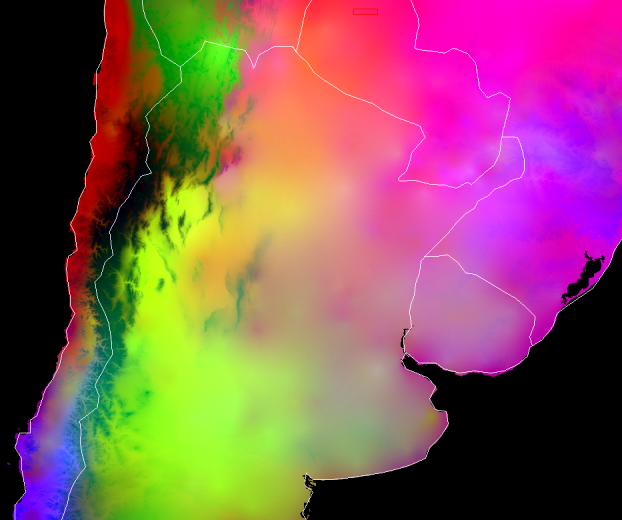
\includegraphics[width=0.6\textwidth]{images/temp_prec}%
      \caption{RGB: BIO1 = temperatura media anual, BIO7 = rango anual de
              temperatura (BIO5-BIO6) y BIO12 = precipitación anual}\label{fig:temp_prec}
    \end{figure}

    \begin{figure}[hbt]
      \centering%
      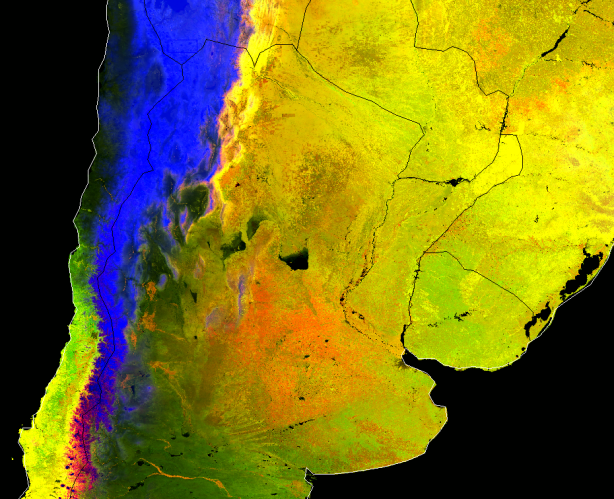
\includegraphics[width=0.6\textwidth]{images/ndvi_dem}%
      \caption{RGB: \textit{NDVI} de \textit{MODIS} promedio Enero, \textit{NDVI} de
               \textit{MODIS} promedio de Julio y DEM}\label{fig:ndvi_dem}
    \end{figure}

    \par De una manera similar, la Figura \ref{fig:ndvi_dem} presenta en RGB el
      \textit{NDVI} de \textit{MODIS} promedio de Enero, \textit{NDVI} de
      \textit{MODIS} promedio de Julio y el \textit{DEM}.

\section{Evaluación de la solución propuesta}

  \begin{figure}[hbt]

    \centering%
    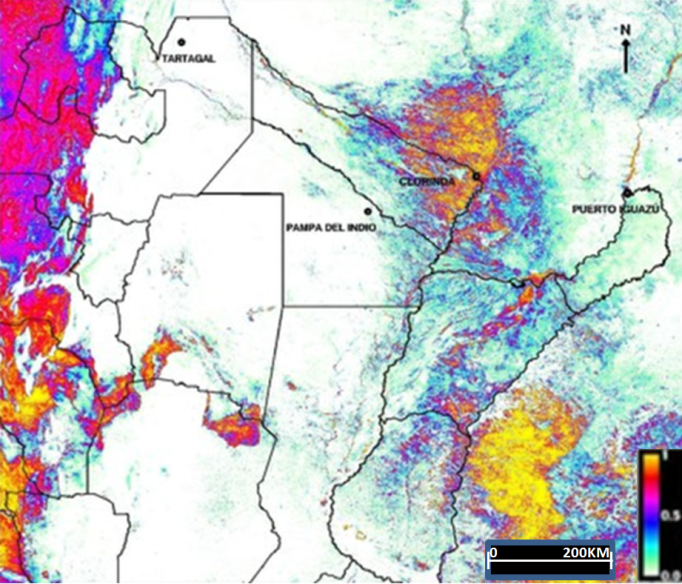
\includegraphics[width=0.6\textwidth]{images/ned_clorinda}%
    \caption{Similaridad ambiental ($\frac{1}{NED}$)
            de cada pixel a las condiciones de Clorinda}\label{fig:ned_clorinda}
  \end{figure}

  \begin{figure}[hbt]
    \centering%
    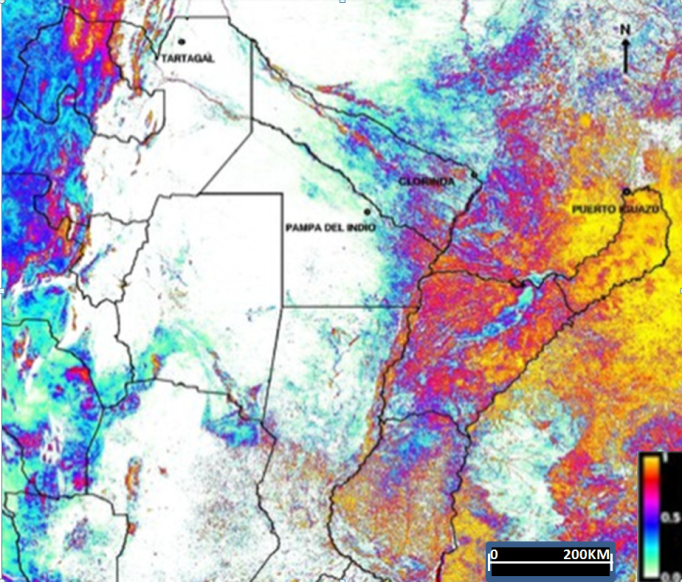
\includegraphics[width=0.6\textwidth]{images/ned_iguazu}%
    \caption{Similaridad ambiental ($\frac{1}{NED}$)
            de cada pixel a las condiciones de Iguazú}\label{fig:ned_iguazu}
  \end{figure}


  \par El resultado de las distancias ambientales normalizadas calculadas de
    cada pixel a cada una de las 4 ciudades se presenta en la Figuras
    \ref{fig:ned_clorinda}, \ref{fig:ned_iguazu}, \ref{fig:ned_pampa} y
    \ref{fig:ned_tartagal}. Es importante tener en cuenta que la inversa de Distancia Ambiental
    Normalizada ($\frac{1}{NED}$) nos dice qué tan similar es una ciudad en
    comparación con las otras tres.
    \begin{figure}[hbt]
      \centering%
      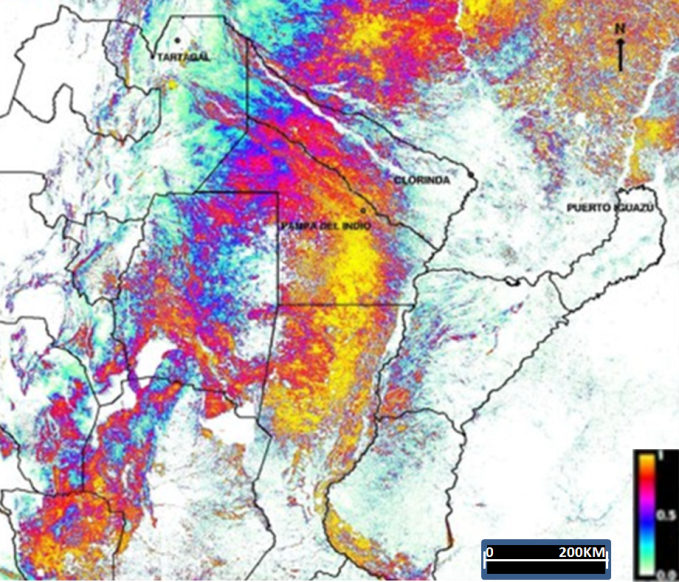
\includegraphics[width=0.6\textwidth]{images/ned_pampa}%
      \caption{Similaridad ambiental ($\frac{1}{NED}$)
              de cada pixel a las condiciones de Pampa del Indio}\label{fig:ned_pampa}
    \end{figure}


    \begin{figure}[hbt]
      \centering%
      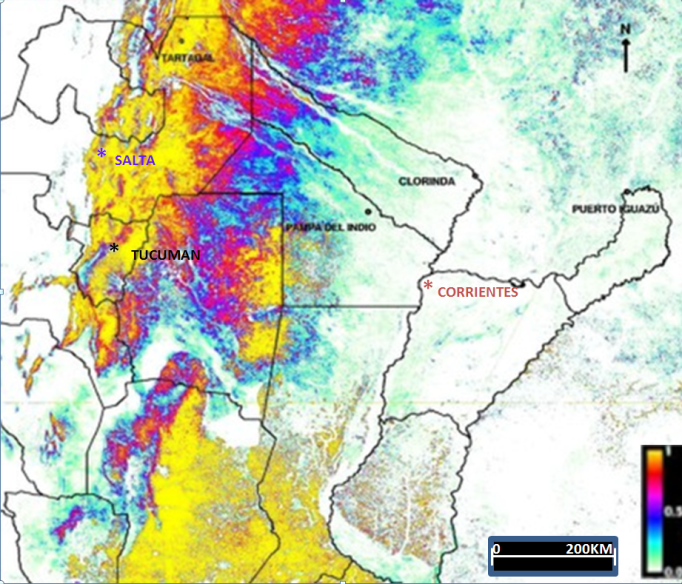
\includegraphics[width=0.6\textwidth]{images/ned_tartagal}%
      \caption{Similaridad ambiental ($\frac{1}{NED}$)
              de cada pixel a las condiciones de Tartagal.
              Aquí también se incluyen las localizaciones de las tres ciudades
              tomadas como ejemplo para el cálculo de nuevos modelos
              (Salta, Tucumán, Corrientes)}\label{fig:ned_tartagal}
    \end{figure}

  \par Claramente por estar normalizada, no es una medida de similaridad en
    términos absolutos. Así, por ejemplo en la Figura \ref{fig:ned_iguazu} los
    píxeles con valores
    cercanos a 1 significan que estos lugares son ambientalmente mucho más
    parecidos a Iguazú que a Tartagal o Clorinda o Pampa del Indio.


  \par Sólo como ejemplo, la inversa de la distancia normalizada ($\frac{1}{NED}$)
    de Tucumán, Corrientes y Salta se describen en la Tabla \ref{Tab:comparacion_ned}.
    Estos valores son presentados de una manera diferente en la Figura \ref{fig:ned_contrib}
    donde se intenta graficar con más claridad la contribución que tendrán cada
    uno de los 4 modelos previamente desarrollados, cuando se intenten modelar
    estas 3 nuevas ciudades.
    \begin{figure}[hbt][H]
      \centering%
      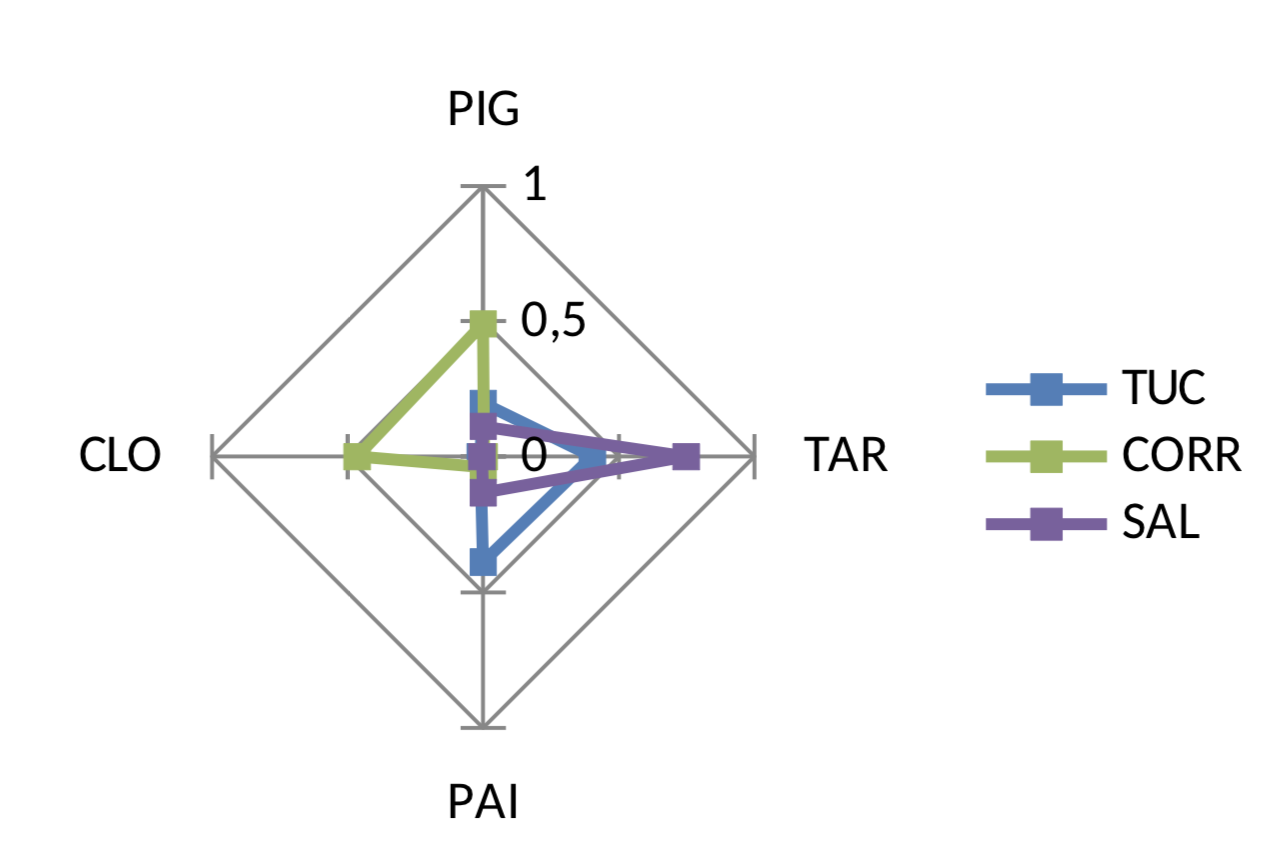
\includegraphics[width=0.6\textwidth]{images/ned_contrib}%
      \caption{Contribución que poseen los modelos para Salta, Corrientes y
              Tucumán de los 4 modelos disponibles}\label{fig:ned_contrib}
    \end{figure}

  \par Para el caso de las tres ciudades simuladas, la distancia ambiental
    realmente tiene una fuerte correlación con la distancia geográfica estándar.
    Estos ejemplos muestran más bien cómo el método funciona, que las ventajas
    que ofrece el mismo. Sin embargo la diferencia entre la distancia ambiental
    y la geográfica puede observarse claramente en las Figuras \ref{fig:ned_clorinda}
    a \ref{fig:ned_tartagal}.
    En todas ellas vemos como la distancia ambiental posee bordes abruptos
    (cosa que la distancia geográfica nunca tendrá).
    Por ejemplo en la Mesopotamia (Figura \ref{fig:ned_iguazu}) o en las yungas
    (Figura \ref{fig:ned_clorinda}) puede verse
    cómo pequeñas distancias geográficas tienen asociadas fuertes gradientes en
    la distancia ambiental (grandes distancias ambientales) y por ende
    podríamos suponer que localidades cercanas geográficamente poseen patrones
    temporales de la población de vectores muy diferentes.

    \begin{table}[hbt]
    \centering
    \caption{Inversa de NED de cuatro ciudades a las 4 localidades predefinidas}\label{Tab:comparacion_ned}
    \begin{tabular}{*7{r}}
    \toprule
    & Puerto Iguazú
    & Clorinda
    & Pampa del Indio
    & Tartagal \\ \midrule
    Tucuman
    &$0.197$
    &$0.011$
    &$0.388$%&\boldmath$1.108$  %CARO: cambio
    &$0.402$\\
    Corrientes
    &$0.491$
    &$0.466$
    &$0.039$
    &$0.002$ \\
    Salta
    &$0.112$
    &$0.005$
    &$0.133$   %CARO: cambio
    &$0.749$ \\
    \bottomrule
    \end{tabular}
    \end{table}

\section{Discusión y propuesta futura}
  \par En el presente capítulo pretendemos generar una contribución al objetivo de
    construir pronósticos dinámicos para la población de vectores,
    utilizando productos satelitales. Se aborda el problema de cómo generalizar
    espacialmente modelos ajustados para ciertas localidades específicas.

  \par Para ello, se propone una metodología basada en ideas ecológicas
    incorporando el concepto de distancia ambiental normalizada.
    Se ha mostrado que el mismo si bien es novedoso es conceptualmente simple.
    Se describe un método simple para calcularlo y ejemplos de su
    implementación especifica de la estimación de este parámetro en
    función de un conjunto de variables ambientales relevantes para la
    ecología del vector del dengue.

  \par Cabe resaltar que esta idea de interpolación ambiental que se
    plantea aquí para modelos relacionados a la epidemiologia,
    podría también ser utilizados a la hora de contar con datos
    puntuales de otras variables (por ejemplo rendimiento en la producción
    agrícola) donde la distancia espacial no refleje tan adecuadamente la
    similaridad entre sitios como lo es la distancia ambiental.


  \par Los resultados y metodologías aquí planteadas fueron presentadas en el
    \textit{Congreso Bienal de IEEE Argentina} (ARGENCON) durante la primer semana de Junio
    de 2018. La presentación fue realizada bajo el título
    \textit{Generalización espacial de modelos epidemiológicos basada en el
    concepto de Distancia Ambiental Normalizada NED} \cite{ned_scavuzzo} y
    se podrá encontrar en la \textit{IEEE Xplore Digital Library} (\url{https://ieeexplore.ieee.org/}).
%\end{document}
